\documentclass[a4paper,11pt]{article}
\usepackage{sbpo-template}
%\usepackage[latin1]{inputenc}
\usepackage[brazil]{babel}    % português do Brasil
\usepackage[utf8]{inputenc}   % acentos no UTF-8
\usepackage[T1]{fontenc}      % para hifenização correta
\usepackage{amsmath,amssymb}
\usepackage{url}
\usepackage{float}
\usepackage[square]{natbib}
\usepackage{indentfirst}
\usepackage{fancyhdr}
\usepackage{graphicx}
\pagestyle{fancy}
\fancyhf{}
\fancyhead[C]{
\includegraphics[scale=0.5]{sbpo2026-header-logo.png}}
%\renewcommand{\headrulewidth}{0pt}
\renewcommand{\headruleskip}{-1mm}
%\setlength\headheight{101.0pt}
%\addtolength{\textheight}{-101.0pt}
\setlength\headheight{86pt}
\addtolength{\textheight}{-86pt}
\setlength{\headsep}{5mm}
\setlength{\footskip}{4.08003pt}
\usepackage[section]{placeins}

%TO DO:
% Acrescentar uma revisão de literatura mais bem estruturada e explicativa. 
% Desenvolver melhor a discussão dos resultados para além do que está visível nas tabelas e gráficos). 
% Corrigir as citações que não estão separadas por colchetes (quando não fazem parte direta do texto). 
% Estruturar melhor o resumo e evitar siglas sem explicação.

\begin{document}

\title{Análise do Impacto do Carregamento Paralelo de Dados no Treinamento de Redes Neurais Convolucionais} 

\maketitle
\thispagestyle{fancy}

\author{
\name{Antonio Ambrosio da Silva}
\institute{Instituto Federal de Educação, Ciência e Tecnologia de Minas Gerais (IFMG) – Campus Bambuí, Bambuí, MG, Brasil.}
\email{antonioambrosiooficial@gmail.com}
}

\author{ 
\name{Euler Gomes da Rocha}
\institute{Instituto Federal de Educação, Ciência e Tecnologia de Minas Gerais (IFMG) – Campus Bambuí, Bambuí, MG, Brasil.} 
\email {eulergomesrocha@gmail.com}
}

\author{ 
\name{Vinícius Miguel Leite Gomes de Souza}
\institute{Instituto Federal de Educação, Ciência e Tecnologia de Minas Gerais (IFMG) – Campus Bambuí, Bambuí, MG, Brasil.} 
\email {viniciusmiguellgds@gmail.com}
}

\author{
\name{Bruno Alberto Soares Oliveira}
\institute{Grupo de Pessquisa em Sistemas Computacionais, Instituto Federal de Educação, Ciência e Tecnologia de Minas Gerais (IFMG) – Campus Bambuí, Bambuí, MG, Brasil.}
\email{bruno.alberto@ifmg.edu.br}
}

\author{
\name{Ciniro Aparecido Leite Nametala}
\institute{Grupo de Pessquisa em Sistemas Computacionais, Instituto Federal de Educação, Ciência e Tecnologia de Minas Gerais (IFMG) – Campus Bambuí, Bambuí, MG, Brasil.}
\email{ciniro.nametala@ifmg.edu.br}
}

\author{
\name{Marcos Roberto Ribeiro}
\institute{Grupo de Pessquisa em Sistemas Computacionais, Instituto Federal de Educação, Ciência e Tecnologia de Minas Gerais (IFMG) – Campus Bambuí, Bambuí, MG, Brasil.}
\email{marcos.ribeiro@ifmg.edu.br}
}

\vspace{8mm}
\begin{resumo}
Este trabalho analisa como o carregamento paralelo de dados afeta o treinamento de redes neurais para classificação de imagens médicas. Avalia o impacto de num\_workerss e batch\_size em tempo, throughput e acurácia, usando o dataset HAM10000 em um desktop e no Google Colab. Os resultados mostram que o paralelismo pode reduzir significativamente o tempo em até mais de 5 vezes, mas há saturação devido a limitações de hardware. O batch\_size teve impacto menor. Conclui-se que a escolha adequada desses parâmetros e do hardware é essencial para otimizar o treinamento.
\end{resumo}

\bigskip
\begin{palchaves}
Redes Neurais Convolucionais, Paralelismo, Carregamento de Dados, Imagens Médicas
\end{palchaves}


\vspace{8mm}

\begin{abstract}
This work analyzes how parallel data loading affects the training of neural networks for medical image classification. It evaluates the impact of num\_workerss and batch\_size on time, throughput, and accuracy, using the HAM10000 dataset on a desktop and on Google Colab. The results show that parallelism can significantly reduce training time by more than 5 times, but there is saturation due to hardware limitations. The batch\_size had a smaller impact. It is concluded that the proper choice of these parameters and the hardware is essential to optimize training.
\end{abstract}

\bigskip
\begin{keywords}
Convolutional Neural Networks, Parallelism, Data Loading, Medical Images.

\end{keywords}

 
\newpage
\section{Introdução} 

O avanço recente das técnicas de aprendizado de máquina, em especial das redes neurais profundas, tem impulsionado aplicações relevantes na área da saúde, como a classificação automática de imagens médicas. Modelos baseados em redes neurais convolucionais (CNNs) têm apresentado alto desempenho em tarefas como detecção de doenças em exames de imagem, contribuindo para apoio ao diagnóstico clínico \cite{lecun2015deep, krizhevsky2012imagenet}.

Entretanto, o treinamento desses modelos envolve grande volume de dados e elevado custo computacional, tornando-se um desafio relevante em termos de desempenho e eficiência. Uma parte significativa desse custo está associada ao carregamento e pré-processamento dos dados, que pode se tornar um gargalo no pipeline de treinamento \cite{goodfellow2016deep}.

Nesse contexto, técnicas de paralelismo têm sido amplamente exploradas para reduzir o tempo de treinamento. Em particular, o uso de múltiplos processos para carregamento de dados, como implementado no parâmetro \textit{num\_workerss} do DataLoader em bibliotecas como o \textit{PyTorch}, permite que operações de leitura e transformação de dados sejam realizadas de forma concorrente, potencialmente aumentando o \textit{throughput} do sistema.

A análise do impacto do paralelismo pode ser fundamentada pela Lei de Amdahl, que estabelece limites teóricos para o ganho de desempenho em sistemas paralelos, considerando a fração do código que permanece sequencial \cite{amdahl1967validity}. De acordo com essa lei, o ganho obtido com paralelização é limitado pela parte não paralelizável do processo, o que torna essencial a análise experimental do comportamento do sistema.

Dessa forma, este trabalho tem como objetivo investigar como o carregamento paralelo de dados influencia o desempenho do treinamento de redes neurais convolucionais aplicadas à classificação de imagens médicas. Para isso, são conduzidos experimentos variando o número de processos de carregamento (\textit{num\_workerss}) e o tamanho do lote (\textit{batch\_size}), avaliando métricas como tempo de treinamento, \textit{throughput} e acurácia do modelo.

Como principal contribuição, este trabalho apresenta uma análise experimental detalhada do impacto do paralelismo no carregamento de dados em diferentes ambientes computacionais, evidenciando limites práticos e diretrizes para otimização do treinamento de redes neurais.

\section{Trabalhos Relacionados}


% Relacionar a Lei de Amdahl 

O desempenho do treinamento de redes neurais profundas tem sido amplamente estudado, especialmente no contexto de grandes volumes de dados e alto custo computacional. Estudos recentes mostram que, além do modelo em si, o pipeline de dados exerce papel fundamental no tempo total de treinamento, podendo se tornar um gargalo significativo \cite{mohan2020analyzing}.

Nesse sentido, diversos trabalhos investigam o impacto do carregamento de dados no desempenho de modelos de aprendizado profundo. \cite{svogor2022profiling} analisam o funcionamento do DataLoader do PyTorch em ambientes com alta latência de armazenamento, demonstrando que otimizações no carregamento podem reduzir significativamente o tempo de treinamento, alcançando melhorias de até 12 vezes em determinados cenários. De forma semelhante, \cite{sun2022solar} propõem um novo mecanismo de carregamento de dados para treinamento distribuído, obtendo ganhos expressivos de desempenho ao otimizar o acesso e o paralelismo no sistema de I/O.

Além disso, \cite{mohan2020analyzing} demonstram que o tempo de treinamento de redes neurais pode ser fortemente impactado por períodos de espera por dados, conhecidos como \textit{data stalls}, evidenciando a importância de otimizar o pipeline de entrada. Os autores mostram que, em alguns casos, o tempo de espera por dados pode dominar o tempo total de execução.

No contexto de frameworks de aprendizado profundo, estudos como o de \cite{aach2023large} analisam o desempenho de diferentes abordagens de treinamento distribuído, destacando a importância da paralelização para lidar com grandes volumes de dados e melhorar a escalabilidade dos modelos.

Especificamente no PyTorch, o parâmetro \textit{num\_workerss} do DataLoader permite o carregamento paralelo de dados por meio de múltiplos processos. O uso adequado desse parâmetro pode aumentar o throughput do sistema ao permitir que o carregamento e o processamento de dados ocorram simultaneamente com o treinamento do modelo \cite{svogor2022profiling}. No entanto, o aumento do número de processos também pode introduzir overhead e competição por recursos, o que pode limitar os ganhos de desempenho.

Dessa forma, a literatura evidencia que o carregamento de dados é um componente crítico no treinamento de redes neurais profundas, sendo necessário encontrar um equilíbrio entre paralelismo e custo computacional. Este trabalho se insere nesse contexto, investigando experimentalmente o impacto do parâmetro \textit{num\_workerss} e do tamanho do lote no desempenho do treinamento de modelos de classificação de imagens médicas.

\section{Metodologia}

A metodologia adotada neste trabalho tem como objetivo avaliar o impacto do paralelismo no carregamento de dados durante o treinamento de redes neurais convolucionais. Para isso, foram conduzidos experimentos controlados variando o número de workers do \textit{DataLoader} e o tamanho do \textit{batch}, analisando seu efeito no desempenho do treinamento.

\subsection{Preparação dos Dados}

Foi utilizado o dataset HAM10000, composto por aproximadamente 10.000 imagens de lesões de pele distribuídas em sete classes. As imagens foram organizadas em diretórios compatíveis com a estrutura esperada pela classe \textit{ImageFolder} da biblioteca PyTorch. 

\begin{figure}[H]
    \centering
    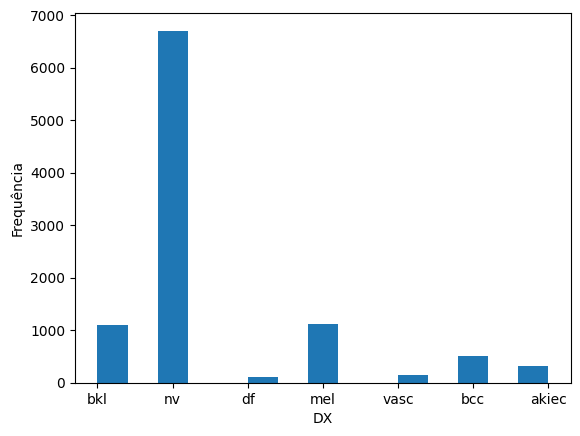
\includegraphics[width=0.7\textwidth]{images/dataset.png}
    \caption{Histograma do dataset}
    \small{Fonte: Autores (2026)}
    \label{fig:hist_data}
\end{figure}

A figura \ref{fig:hist_data} representa o histograma do \textit{dataset}, mostrando a recorrência das sete classes presentes. 
Nota-se que há um desbalanceamento entre as classes presentes, onde a classe 'nv' apresenta uma recorrência significativamente maior do que as outras classes.

As imagens passaram por um processo de pré-processamento utilizando \texttt{torchvision.transforms}, incluindo redimensionamento para 128×128 pixels, conversão para tensor e normalização dos valores de pixel. Essas transformações garantem compatibilidade com o modelo e contribuem para a estabilidade do treinamento.

O conjunto de dados foi dividido em subconjuntos de treino e validação, permitindo a avaliação do desempenho do modelo durante o processo de aprendizado.


\subsection{Implementação da Função de Treinamento}

Foi implementada uma função de treinamento parametrizada que recebe como entrada o número de workers (\texttt{num\_workerss}) e o tamanho do lote (\texttt{batch\_size}). Essa função é responsável por:

\begin{itemize}
    \item Criar os \textit{DataLoaders} de treino e validação com os parâmetros especificados;
    \item Inicializar o modelo de rede neural convolucional;
    \item Definir o otimizador Adam com taxa de aprendizado de 0.001;
    \item Utilizar a função de perda \textit{CrossEntropyLoss};
    \item Executar o treinamento por 5 épocas;
    \item Medir métricas de desempenho, incluindo tempo por época, tempo total, throughput (imagens por segundo) e acurácia no conjunto de validação.
\end{itemize}

O modelo utilizado consiste em uma rede neural convolucional com três camadas convolucionais, seguidas por camadas de \textit{pooling}, camadas totalmente conectadas e uma camada de \textit{dropout} para reduzir \textit{overfitting}.

\subsection{Experimentos}

Os experimentos foram organizados em duas etapas principais, com o objetivo de analisar separadamente o impacto do paralelismo no carregamento de dados e a influência do tamanho do lote no desempenho do treinamento.

\subsubsection{Variação do Número de Workers}

Nesta etapa, o tamanho do \textit{batch} foi mantido fixo em 64, enquanto o número de workers do \textit{DataLoader} foi variado entre os valores de 0, 2, 4, 6 e 8.

Para cada configuração, foram coletadas métricas como tempo por época, tempo total, throughput e acurácia. 
Cada experimento foi realizado com um modelo inicializado com pesos aleatórios, garantindo independência entre os testes.
O objetivo foi avaliar como o paralelismo no carregamento de dados influencia o desempenho do treinamento.


\subsubsection{Variação do Batch Size}

Na segunda etapa, o número de workers foi fixado em um valor intermediário (tipicamente 4), enquanto o tamanho do \textit{batch} foi variado entre os valores de 32, 64, 128 e 256, quando permitido pela memória disponível.

Para os testes variando o tamanho do \textit{batch}, foi seguido o mesmo padrão da etapa anterior, coletando as mesmas métricas e gerando um novo modelo por valor de \textit{batch}.
Essa análise permitiu investigar a relação entre o tamanho do lote e o desempenho computacional, bem como sua interação com o paralelismo no carregamento de dados.

\subsection{Materiais e tecnologias}\label{MT}

A implementação foi realizada na linguagem de programação Python (versão 3.11) \cite{python} em conjunto com o ambiente interativo Jupyter Notebook \cite{jupyter}.
Para a construção do modelo foi utilizado a biblioteca de código aberto Pytorch \cite{pytorch}

Para melhores testes e verificação do funcionamento do projeto, foram utilizados dois diferentes \textit{hardwares}, sendo eles: 
\begin{itemize}
    \item Um computador \textit{Desktop} com um AMD Ryzen 5 7600X, 32GB de memória RAM e uma placa de vídeo NVIDIA RTX 5070, que conta com 6.144 núcleos CUDA.
    \item A ferramenta gratuita em nuvem Google Colab, que conta com uma NVIDIA Tesla T4, que conta com 2.560 núcleos CUDA.
\end{itemize}

Ambos os dois diferentes hardwares foram testados utilizando o mesmo código-fonte, para garantir a equiparidade dos resultados.

\section{Resultados e Discussão}

Nesta seção, são apresentados e analisados os resultados obtidos para cada configuração de hardware descrita na Seção \ref{MT}, com foco no impacto dos parâmetros \textit{num\_workerss} e \textit{batch\_size} no desempenho e na acurácia do modelo.


\subsection{Hardware 1}

Utilizando o Hardware 1 (desktop equipado com processador AMD Ryzen 5 7600X, 32 GB de memória RAM e GPU NVIDIA RTX 5070), observou-se um impacto significativo do paralelismo no carregamento de dados sobre o desempenho do treinamento.

%EULER
\begin{table}[H]
\centering
\begin{tabular}{|l|l|l|l|l|}
\hline
num\_workers & Tempo/época (s) & Tempo total(s) & Throughput (img/s) & Acurácia (\%) \\ \hline
0           &  21.66          &     110.13     &    316,95          &   74,90      \\ \hline
2           &  11.36          &     56.79      &    614.59          &   74,13      \\ \hline
4           &  6.24           &     31.18      &    1119.44         &   74,90      \\ \hline
6           &  4.55           &     22.89      &    1524.91         &   74,59      \\ \hline
8           &  4.09           &     20.73      &    1683.77         &   73,71     \\ \hline
\end{tabular}
\caption{Variação de num\_workerss (batch\_size=64)}
\label{tab:num_workers_e}
\end{table}

Conforme apresentado na Tabela \ref{tab:num_workers_e}, o aumento do parâmetro \textit{num\_workerss} de 0 para 8 resultou em uma redução expressiva no tempo por época, passando de 21,66 s para 4,09 s, o que corresponde a um ganho superior a 80\%. De forma consistente, o \textit{throughput} aumentou de 316,95 para 1683,77 imagens por segundo, evidenciando a mitigação do gargalo de entrada/saída (I/O) por meio do carregamento paralelo de dados.

Entretanto, observa-se um comportamento de saturação nos ganhos de desempenho. A partir de 6 \textit{workers}, a redução no tempo por época torna-se marginal, indicando que outros componentes do sistema passam a limitar o desempenho global, como CPU, largura de banda de memória e comunicação com a GPU. Esse comportamento está em conformidade com a Lei de Amdahl, que estabelece limites para o ganho de desempenho em sistemas paralelos.

Em relação à acurácia, os resultados permaneceram estáveis, variando entre 73\% e 75\%, indicando que o aumento do paralelismo no carregamento de dados não impacta significativamente a qualidade do modelo, mas apenas o tempo de treinamento.


\begin{table}[H]
\centering
\begin{tabular}{|l|l|l|l|}
\hline
batch\_size & Tempo/época (s) & Throughput (img/s) & Acurácia (\%) \\ \hline
32          & 5.84            &   1175.18          &  74.72       \\ \hline
64          & 6.20            &   1136.05          &  73.81       \\ \hline
128         & 6.09            &   1141.43          &  74.82       \\ \hline
256         & 6.20            &   1120.25          &  72.53       \\ \hline
\end{tabular}
\caption{Variação de batch\_size (num\_workerss=4)}
\label{tab:batch_size_e}
\end{table}

No que se refere ao tamanho do lote (Tabela \ref{tab:batch_size_e}), observa-se que a variação do \textit{batch\_size} não resultou em mudanças expressivas no tempo por época nem no \textit{throughput}, cujos valores permaneceram próximos em todas as configurações avaliadas.

Por outro lado, a acurácia apresentou pequenas variações, com melhor resultado obtido para \textit{batch\_size} 128 (74,82\%), sugerindo um possível equilíbrio entre estabilidade do gradiente e eficiência computacional. Valores muito elevados de \textit{batch\_size}, como 256, apresentaram leve queda de desempenho em termos de generalização.

\begin{figure}[!htb]
    \centering
    \includegraphics[width=0.7\textwidth]{images/TrxN_E.png}
    \caption{Evolução do \textit{throughput} em função do número de \textit{workers}, evidenciando ponto de saturação do paralelismo}
    \small{Fonte: Autores (2026)}
    \label{fig:trxne}
\end{figure}

A Figura \ref{fig:trxne} ilustra o comportamento do \textit{throughput} em função do número de \textit{workers}, evidenciando um crescimento acentuado até 6 \textit{workers}, seguido de estabilização. Esse resultado reforça a presença de um ponto de saturação do sistema.

\FloatBarrier
\clearpage

\begin{figure}[!htb]
    \centering
    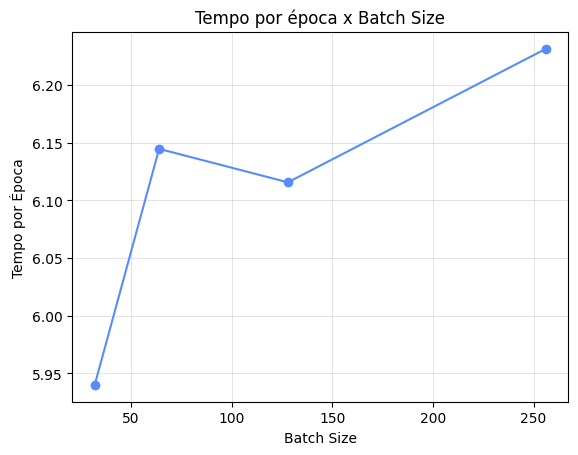
\includegraphics[width=0.7\textwidth]{images/TxB_E.png}
    \caption{Tempo por época em função do \textit{batch\_size}, evidenciando baixa sensibilidade do desempenho}
    \small{Fonte: Autores (2026)}
    \label{fig:txbe}
\end{figure}

A Figura \ref{fig:txbe} apresenta o tempo por época em função do \textit{batch\_size}, indicando variações pouco significativas entre as configurações, com leve vantagem para o valor 128.

\FloatBarrier

\begin{figure}[!htb]
    \centering
    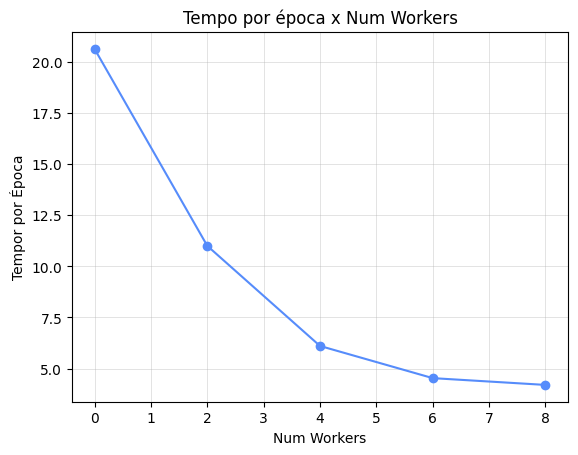
\includegraphics[width=0.7\textwidth]{images/TxN_E.png}
    \caption{Tempo por época em função do número de \textit{workers}, evidenciando redução inicial seguida de saturação}
    \small{Fonte: Autores (2026)}
    \label{fig:txne}
\end{figure}

Por fim, a Figura \ref{fig:txne} demonstra a redução do tempo por época com o aumento de \textit{num\_workerss}, sendo o melhor resultado obtido com 8 \textit{workers}, ainda que com ganhos marginais em relação a 6.


\FloatBarrier
Esse comportamento experimental está diretamente alinhado com a Lei de Amdahl, evidenciando que, à medida que a fração paralelizável do sistema é explorada, o ganho adicional de desempenho torna-se limitado pela porção sequencial do pipeline.

De forma geral, os resultados indicam que, para o hardware analisado, o parâmetro \textit{num\_workerss} exerce influência significativamente maior sobre o desempenho do que o \textit{batch\_size}, sendo um fator crítico para a otimização do tempo de treinamento.

 
\subsection{Hardware 2}

Utilizando o Hardware 2 (ambiente Google Colab com GPU NVIDIA Tesla T4), os resultados apresentaram comportamento distinto em relação ao Hardware 1, especialmente no que se refere ao paralelismo no carregamento de dados.

%VINICIUS
\begin{table}[H]
\centering
\begin{tabular}{|l|l|l|l|l|}
\hline
num\_workers & Tempo/época (s) & Tempo total (s) & Throughput (img/s) & Acurácia (\%) \\ \hline
0           & 53,15           & 265,79          & 131,33             & 74,59         \\ \hline
2           & 43,12           & 215,58          & 161,91             & 75,26         \\ \hline
4           & 43,57           & 217,86          & 160,22             & 74,17         \\ \hline
6           & 44,02           & 220,12          & 158,57             & 73,81         \\ \hline
8           & 45,56           & 227,79          & 153,24             & 73,74         \\ \hline
\end{tabular}
\caption{Variação de num\_workerss (batch\_size=64)}
\label{tab:num_workersv}
\end{table}

De acordo com a Tabela \ref{tab:num_workersv}, o aumento de \textit{num\_workerss} de 0 para 2 proporcionou melhora significativa no desempenho, com redução do tempo por época de 53,15 s para 43,12 s e aumento do \textit{throughput} de 131,33 para 161,91 imagens por segundo.

Entretanto, a partir desse ponto, o aumento adicional do número de \textit{workers} não resultou em ganhos, sendo observado inclusive um leve aumento no tempo de execução para valores superiores a 4 \textit{workers}. Esse comportamento indica que o sistema atinge rapidamente um ponto de saturação, no qual o custo de gerenciamento de múltiplos processos e a contenção de recursos superam os benefícios do paralelismo.

Esse efeito pode estar associado às limitações do ambiente do Google Colab, como restrições de CPU, menor controle sobre recursos de hardware, contenção em memória compartilhada e possíveis limitações de I/O.

Em relação à acurácia, os valores permaneceram estáveis entre 73\% e 75\%, com melhor desempenho observado para 2 \textit{workers}, reforçando que o paralelismo impacta principalmente o tempo de execução, sem afetar significativamente a qualidade do modelo.


\begin{table}[H]
\centering
\begin{tabular}{|l|l|l|l|}
\hline
batch\_size & Tempo/época (s) & Throughput (img/s) & Acurácia (\%) \\ \hline
32          & 44,10           & 158,30             & 75,03         \\ \hline
64          & 43,46           & 160,62             & 74,72         \\ \hline
128         & 43,34           & 161,08             & 74,34         \\ \hline
256         & 44,66           & 156,31             & 71,75         \\ \hline
\end{tabular}
\caption{Variação de batch\_size (num\_workerss=4)}
\label{tab:batch_sizev}
\end{table}

Na análise do \textit{batch\_size} (Tabela \ref{tab:batch_sizev}), o tempo por época e o \textit{throughput} permaneceram praticamente constantes entre as configurações, com pequenas variações. O maior \textit{throughput} foi obtido com \textit{batch\_size} 128, enquanto a maior acurácia foi observada com \textit{batch\_size} 32 (75,03\%).

Por outro lado, o aumento do \textit{batch\_size} para 256 resultou em queda significativa da acurácia (71,75\%), o que pode estar relacionado à redução da frequência de atualização dos pesos e à possível degradação da capacidade de generalização do modelo.


\begin{figure}[!htb]
    \centering
    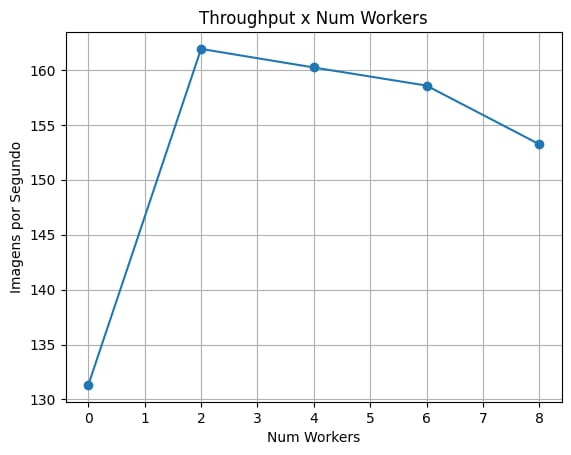
\includegraphics[width=0.7\textwidth]{images/TRxN_V.jpeg}
    \caption{Evolução do \textit{throughput} em função do número de \textit{workers}, evidenciando ponto de saturação do paralelismo}
    \small{Fonte: Autores (2026)}
    \label{fig:trxnv}
\end{figure}

A Figura \ref{fig:trxnv} apresenta o comportamento do \textit{throughput} em função do número de \textit{workers}.
Observa-se um crescimento significativo no throughput ao aumentar de 0 para 2 \textit{workers}, passando de aproximadamente 131 para 162 imagens por segundo, o que reforça a hipótese de eliminação de gargalos de I/O.
Após esse ponto, o \textit{throughput} passa a apresentar uma tendência de queda gradual, indicando que o aumento do paralelismo não se traduz em maior eficiência. 

\FloatBarrier
\clearpage

\begin{figure}[!htb]
    \centering
    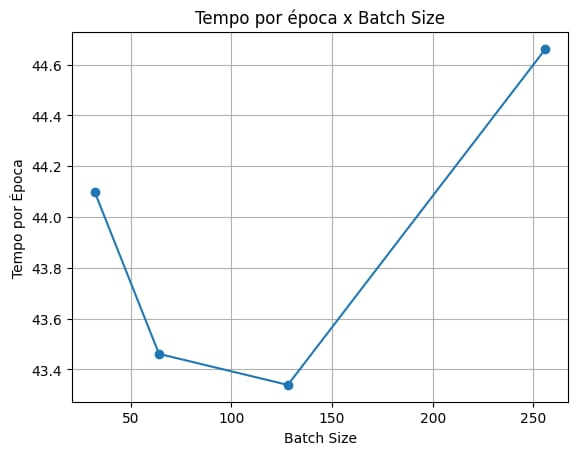
\includegraphics[width=0.7\textwidth]{images/TxB_V.jpeg}
    \caption{Tempo por época em função do \textit{batch\_size}, evidenciando baixa sensibilidade do desempenho}
    \small{Fonte: Autores (2026)}
    \label{fig:txbv}
\end{figure}

A Figura \ref{fig:txbv} apresenta o impacto do tamanho do lote (\textit{batch\_size}) no tempo por época.
Os resultados mostram que o tempo por época apresenta baixa sensibilidade à variação do tamanho do lote, mantendo-se relativamente estável entre os valores analisados. Observa-se uma leve redução até o \textit{batch\_size} 128, onde é atingido o menor tempo médio.

\FloatBarrier

\begin{figure}[!htb]
    \centering
    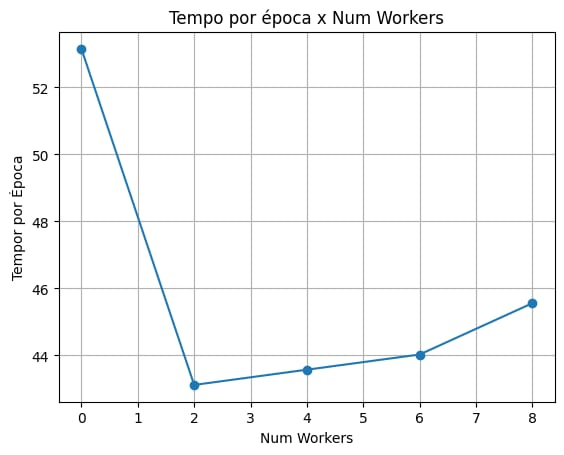
\includegraphics[width=0.7\textwidth]{images/TxN_V.jpeg}
    \caption{Tempo por época em função do número de \textit{workers}, evidenciando redução inicial seguida de saturação}
    \small{Fonte: Autores (2026)}
    \label{fig:txnv}
\end{figure}

A Figura \ref{fig:txnv} apresenta a variação do tempo por época em função do número de \textit{workers}.
Observa-se uma redução acentuada no tempo de execução ao passar de 0 para 2 \textit{workers}, indicando que o paralelismo inicial no carregamento de dados elimina um gargalo significativo de entrada/saída.
Entretanto, a partir de 2 \textit{workers}, verifica-se uma inversão de tendência, com aumento gradual do tempo por época conforme o número de \textit{workers} cresce.


\FloatBarrier

De forma geral, os resultados indicam que, em ambientes com recursos mais limitados ou compartilhados, como o Google Colab, o uso excessivo de paralelismo pode ser contraproducente, sendo recomendada a utilização de um número moderado de \textit{workers} para obtenção do melhor desempenho.

\subsection{Comparação entre os Hardwares}

A comparação entre os dois ambientes experimentais evidencia diferenças significativas no comportamento do paralelismo. No Hardware 1, observou-se escalabilidade mais eficiente com o aumento do número de \textit{workers}, com ganhos expressivos de desempenho até a região de saturação.

Por outro lado, no ambiente do Google Colab (Hardware 2), o ponto de saturação foi atingido precocemente, com melhor desempenho obtido com apenas 2 \textit{workers}. O aumento adicional do paralelismo resultou em degradação de desempenho, indicando maior sensibilidade à contenção de recursos.

Esses resultados demonstram que a eficiência do paralelismo está diretamente relacionada às características do hardware, como número de núcleos de CPU, largura de banda de memória e desempenho do subsistema de I/O. Dessa forma, a escolha do valor de \textit{num\_workerss} deve ser realizada de forma empírica e dependente do ambiente de execução.

\section{Conclusão}

Este trabalho investigou o impacto do carregamento paralelo de dados no desempenho do treinamento de redes neurais convolucionais aplicadas à classificação de imagens médicas. Através de experimentos controlados, foi possível analisar a influência dos parâmetros \textit{num\_workerss} e \textit{batch\_size} em diferentes configurações de hardware.

Os resultados demonstraram que o uso de múltiplos \textit{workers} no \textit{DataLoader} pode reduzir significativamente o tempo de treinamento, aumentando o \textit{throughput} do sistema de forma expressiva. Em particular, no hardware de maior desempenho, observou-se ganhos superiores a 5 vezes quando comparado à execução sequencial. No entanto, também foi identificado um ponto de saturação, no qual o aumento adicional de \textit{workers} resulta em ganhos marginais, evidenciando limitações impostas por recursos não paralelizáveis, conforme previsto pela Lei de Amdahl.

Por outro lado, a variação do \textit{batch\_size} apresentou impacto menos significativo no desempenho computacional, embora pequenas variações na acurácia tenham sido observadas, sugerindo a existência de um compromisso entre eficiência e qualidade do treinamento.

Além disso, os experimentos realizados em diferentes hardwares evidenciam que o ganho obtido com paralelismo depende diretamente das características da máquina, como número de núcleos de CPU, capacidade de memória e desempenho de I/O.

Dessa forma, conclui-se que a otimização do pipeline de dados e o \textit{hardware} utilizado são fatores essenciais para o treinamento eficiente de redes neurais profundas, sendo o ajuste adequado do parâmetro \textit{num\_workerss} uma estratégia simples, porém altamente eficaz, para a melhoria do desempenho em pipelines de treinamento baseados em aprendizado profundo.

Como trabalhos futuros, sugere-se a investigação de técnicas mais avançadas de paralelismo, como pré-busca (\textit{prefetching}), uso de memória compartilhada, armazenamento em SSD de alta velocidade e treinamento distribuído em múltiplas GPUs, bem como a avaliação em datasets maiores e modelos mais complexos.

\section{Agradecimentos}
Os autores agradecem ao Instituto Federal de Educação, Ciência e Tecnologia de Minas Gerais (IFMG) pelo apoio institucional, bem como à Fundação de Amparo à Pesquisa do Estado de Minas Gerais (FAPEMIG), à Coordenação de Aperfeiçoamento de Pessoal de Nível Superior (CAPES) e ao Conselho Nacional de Desenvolvimento Científico e Tecnológico (CNPq) pelo apoio ao desenvolvimento da pesquisa científica no Brasil.

\section*{Disponibilidade de Dados e Código} 

Para fins de transparência e reprodutibilidade científica, o código-fonte da rede, os \textit{scripts} de treinamento e o conjunto de dados estão disponíveis publicamente no repositório GitHub em: \url{https://github.com/eulergomees/parallel_loading}.

O repositório está estruturado com diretórios de suporte, arquivos de requisitos (\textit{requirements.txt}), modelos pré-treinados e um \textit{Jupyter Notebook} detalhando todas as etapas da implementação em Python e PyTorch.

~\\
\bibliographystyle{sbpo}
\bibliography{exemplo-latex}


\end{document}

